\section{Does learned entry sizing improve returns?}\label{sec:12}

\begin{figure}[!htbp]\centering
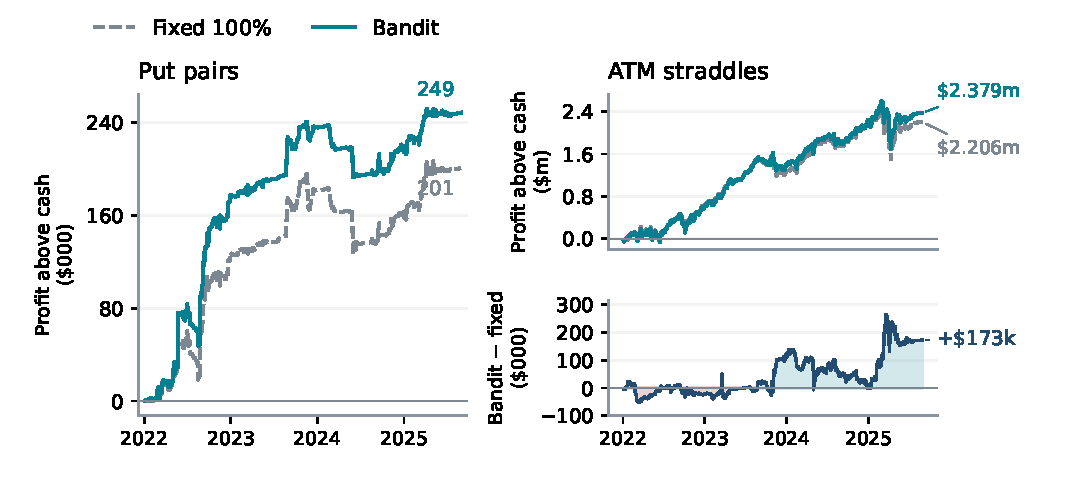
\includegraphics[width=\linewidth]{entry_curves.pdf}
\caption{Profit above cash since January 2022. Upper right: total straddle profits. Lower right: incremental straddle profit, bandit minus fixed full sizing. Series subtract their 2021 closing values and retain carried positions. Differences reflect both sizing and admission.}\label{fig:entry-curves}
\end{figure}

\begin{table}[H]\centering\small
\caption{Entry-sizing policies in validation and later evaluation.}
\setlength{\tabcolsep}{4pt}\renewcommand{\arraystretch}{1.18}
\begin{tabularx}{\textwidth}{@{}>{\hsize=1.66992\hsize\linewidth=\hsize\raggedright\arraybackslash}X>{\hsize=0.81055\hsize\linewidth=\hsize\raggedleft\arraybackslash}X>{\hsize=0.81055\hsize\linewidth=\hsize\raggedleft\arraybackslash}X>{\hsize=0.73242\hsize\linewidth=\hsize\raggedleft\arraybackslash}X>{\hsize=0.97656\hsize\linewidth=\hsize\raggedleft\arraybackslash}X@{}}\toprule
\textbf{Entry policy} & \textbf{2018--21 S} & \textbf{2022--25 S} & \textbf{Later entries} & \textbf{Later profit}\\\midrule
Put pair \(\cdot\) 50\% & 0.437 & 1.007 & 151 & \$0.205m\\
Put pair \(\cdot\) 75\% & 0.449 & 0.944 & 104 & \$0.195m\\
Put pair \(\cdot\) 100\% & 0.478 & 1.055 & 75 & \$0.201m\\
Put pair \(\cdot\) Bandit & 0.573 & 1.263 & 110 & \$0.249m\\
Straddle \(\cdot\) 50\% & 0.740 & 0.920 & 1782 & \$1.824m\\
Straddle \(\cdot\) 75\% & 0.542 & 0.968 & 1222 & \$2.010m\\
Straddle \(\cdot\) 100\% & 0.528 & 0.990 & 940 & \$2.206m\\
Straddle \(\cdot\) Bandit & 0.775 & 1.041 & 1204 & \$2.379m\\
\bottomrule\end{tabularx}\end{table}

The put bandit improves later excess Sharpe by 0.208 and profit above cash by approximately \$47,800 relative to full size. It admits 110 entries instead of 75. The straddle bandit reaches Sharpe 1.041 and \$2.379 million above cash, compared with 0.990 and \$2.206 million at full size. Its earlier Sharpe also exceeds each fixed-size control. Straddles produce much more dollar profit and daily volatility than the put-pair portfolio, making allocation between them economically consequential.


These are comparisons of complete funded policies. All entry policies receive the same proposal pool---608 put-pair proposals and 35,774 straddle proposals---but size changes contract rounding, outstanding risk and the capacity to admit later opportunities. The resulting entries therefore differ. The findings support useful historical exposure choices; they do not isolate predictive sizing from admission effects.


Most of the put learner's later lead develops in 2022, while 2024 loses ground. Its annualized total account return is 4.667\%; growth relative to cash is 0.530\%. Average reserve is 2.44\% and peak reserve 15.77\%. Cash interest explains much total growth; trading value is measured above cash.
